%-PRÄAMBEL----------------------------------------------------------------
\documentclass[ngerman,11pt,twocolumn,a4paper]{article}

%-Import von Paketen------------------------------------------------------
\usepackage[utf8]{inputenc}
\usepackage{csquotes}
\usepackage{amsmath}
\usepackage{amsfonts}
\usepackage{amssymb}
\usepackage{dsfont}
\usepackage{fancyhdr}
\usepackage[german]{babel}
\usepackage[backend=biber,style=numeric,sorting=none]{biblatex}
\usepackage{graphicx}
\usepackage{float}
\usepackage[dvipsnames]{xcolor}
\usepackage[section]{placeins} %Verhindert Fehlpositionierungen von Text / Abbildungen
\usepackage[skip=0pt, indent=17pt]{parskip}
\usepackage{sectsty}
\usepackage{xurl}
\usepackage[format=hang]{caption}
\usepackage{tikz}
\usepackage{tkz-euclide}
\usepackage{pgfplots}
\usepackage[export]{adjustbox}
\usepackage{titlesec}
%-------------------------------------------------------------------------

%-Seiten-Layout-----------------------------------------------------------
\usepackage[top=2.7cm, bottom=2.8cm, left=2.5cm, right=2.5cm, headheight=20pt]{geometry}
\pagestyle{fancy}
\fancyhead{}
\renewcommand{\headrulewidth}{0pt}
\fancyfoot{}
\fancyfoot[R]{Seite \thepage}
\fancypagestyle{plain}
{%
\fancyhf{} % clear all header and footer fields
\fancyfoot[R]{Seite \thepage} % except the center
	\renewcommand{\headrulewidth}{0pt}
}
\predisplaypenalty=9900
%-------------------------------------------------------------------------

%-Definitionen von Commands / Eigenschaften-------------------------------
\AtBeginDocument{\renewcommand{\abstractname}{Abstract}}
%-------------------------------------------------------------------------

%-Definitionen von Worttrennungen-----------------------------------------
\hyphenation{De-flek-to-me-trie}
\hyphenation{de-flek-to-me-trisch}
\hyphenation{de-flek-to-me-tri-sche}
\hyphenation{De-flek-to-me-tri-sche}
\hyphenation{De-flek-to-me-trisch}
\hyphenation{Re-gis-t-rie-rung}
%-------------------------------------------------------------------------

%-Sonstiges---------------------------------------------------------------
\addbibresource{verweise.bib} %Quellenverzeichnis
\graphicspath{{./kurzfassung_bilder/}} %Bilder
\sectionfont{\raggedright} %Section-Titel linksbündig
\addto\captionsgerman{
	\renewcommand{\figurename}{Abb.} % Abkürzung von Abbildungen
	\renewcommand{\tablename}{Tab.} % Abkürzung von Tabellen
}
\DefineBibliographyStrings{german}{% Letzter Zugriff Text im Quellenverzeichnis
urlseen = {Letzter Zugriff:},
}
\pgfplotsset{compat=1.18} %Für PGF Plots
\usetikzlibrary{shapes.callouts,shapes.geometric,calc,positioning,decorations.markings} % Für Tikz-pictures
%Tikz-Set
\tikzset{midarrow/.style={
        decoration={markings,
            mark= at position 0.5 with {\arrow{Latex[width=3mm]}} ,
        },
        postaction={decorate}
    }
}
\setlength{\intextsep}{3pt plus 2pt}
\titlespacing*{\section}{0pt}{1ex plus 1ex minus .2ex}{2ex plus .2ex}
%-------------------------------------------------------------------------

%-Dokument-Informationen--------------------------------------------------
\author{Vipin Singh}
\title{Kurzfassung der Bachelor-Thesis: Entwicklung eines deflektometrischen Prüfaufbaus für spiegelnde Prüfobjekte}
\date{\today}
%-------------------------------------------------------------------------

%-PRÄAMBEL-Ende-----------------------------------------------------------


% Anmerkungen zum Tex-File:
%	- jeder Satz beginnt in einer neuen Zeile
%-DOKUMENT-Start----------------------------------------------------------
\begin{document}
	% Titel und Abstract nicht in zwei Spalten
	\twocolumn[
	  	\begin{@twocolumnfalse}	
			\maketitle
			
			\begin{abstract}
				\noindent
				Das Ziel der vorliegenden Arbeit ist es, Verfahren zur Sichtprüfung von spiegelnden und transparenten Prüfoberflächen einzuführen und mathematisch zu erklären.
				Dabei wird erklärt, welche Methoden im wissenschaftlichen Gebiet der Deflektometrie eingesetzt werden, um Oberflächen vollständig zu erfassen.
				Zur Bearbeitung des Themas werden transparente Brillengläser und spiegelnde Keramikobjekte analysiert und mit den eingeführten Verfahren automatisiert ausgewertet.
				Die Ergebnisse der Auswertung durch die eingeführten Verfahren zeigten, dass es möglich ist, Anomalien der Oberflächenkrümmung spiegelnder und transparenter Prüfobjekte, wie z. B. Pickel, Dellen, Kratzer oder Gravuren, zu erfassen.
				Dadurch wird es ermöglicht, Oberflächendefekte spiegelnder und transparenter Prüfobjekte zu lokalisieren und qualitative Aussagen der Oberflächenbeschaffenheit zu formulieren.
			\end{abstract}
		\end{@twocolumnfalse}
	]
	
	\section{Einführung} \label{sec:einfuehrung}
	Glänzende Oberflächen faszinieren schon seit langer Zeit zahlreiche Menschen.
	Es gibt Studien, die besagen, dass Menschen die optischen Besonderheiten von glänzenden bzw. spiegelnden Oberflächen instinktiv mit Wasser assoziieren \cite{waterAndShininess}.
	Diese Faszination möchte auch die Industrie in uns anregen.
	So werden z. B. täglich große Karosserieflächen glänzend lackiert.
	Zur Qualitätssicherung ist es unumgänglich, die Prüfung der Oberflächen durch automatisierte Prozesse umzusetzen.
	
	\par
	Die Schwierigkeit der Verfahren sind dabei die störenden Spiegelungen in der Oberfläche, die dafür sorgen, dass man anstelle der Oberfläche ein verzerrtes Bild der Umgebung aufnimmt (siehe Abb. \ref{img:spiegelndeKarosserie}).
	%
	%img:rückseitenreflex
	\begin{figure}[H]
		\centering
		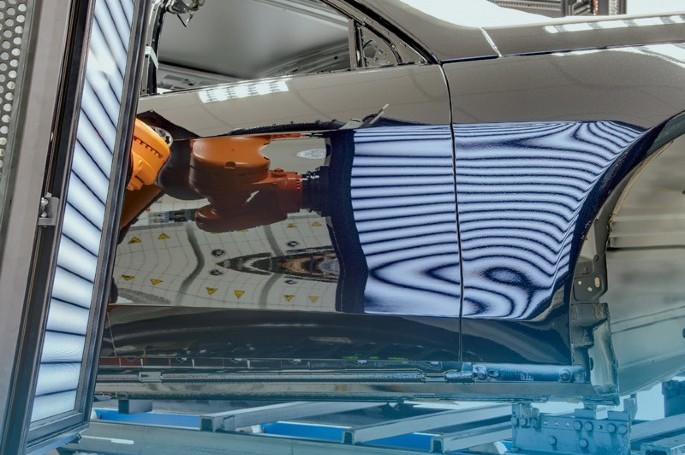
\includegraphics[width=0.75\columnwidth]{spiegelndeKarosserie}
		\caption{Spiegelnde Karosserieoberfläche \cite{spiegelndeKarosserieImg}}
		\label{img:spiegelndeKarosserie}
	\end{figure}	
	
	In dieser Ausarbeitung werden zwei Verfahren vorgeschlagen, um Oberflächendefekte von spiegelnden Prüfobjekten zu erfassen.
	Insbesondere soll dabei auch der Sonderfall für transparente Prüfobjekte behandelt werden.
	
	\section{Grundlagen der Deflektometrie} \label{sec:grundlagenDerDeflektometrie}
	Die Deflektometrie bezeichnet allgemein alle Methoden zur berührungslosen optischen Erfassung von Gestaltinformationen spiegelnder Oberflächen durch automatische Auswertung von Spiegelbildern bekannter Szenen \cite{fraunhofer}.
	Die Szene wird dabei über eine gekrümmte Oberfläche abgelenkt und wird verzerrt im Kamerabild aufgenommen.
	Aus dem Zusammenhang zwischen der Szene und der Spiegelung der Szene auf der spiegelnden Oberfläche können dann Rückschlüssel auf die Oberflächengestalt gezogen werden.
	
	\par
	Eine spiegelnde Oberfläche hat dabei eine lokal glatte Oberflächenbeschaffenheit und reflektiert das auftreffende Licht in eine Richtung.
	Der Sonderfall sind hierbei klare transparente Oberflächen, die zu den spiegelnden Oberflächen gehören.
	Dabei wird das auftreffende Licht nicht nur spekular reflektiert, sondern auch durchgelassen.
	Es können daher Effekte, wie z. B. der Rückseitenreflex auftreten (siehe Abb. \ref{img:rueckseitenreflex}).
	Diese führen zu einer Überlagerung der Spiegelbilder und stören die deflektometrischen Verfahren.
	%
	%img:rueckseitenreflex
	\begin{figure}[H]
		\centering
		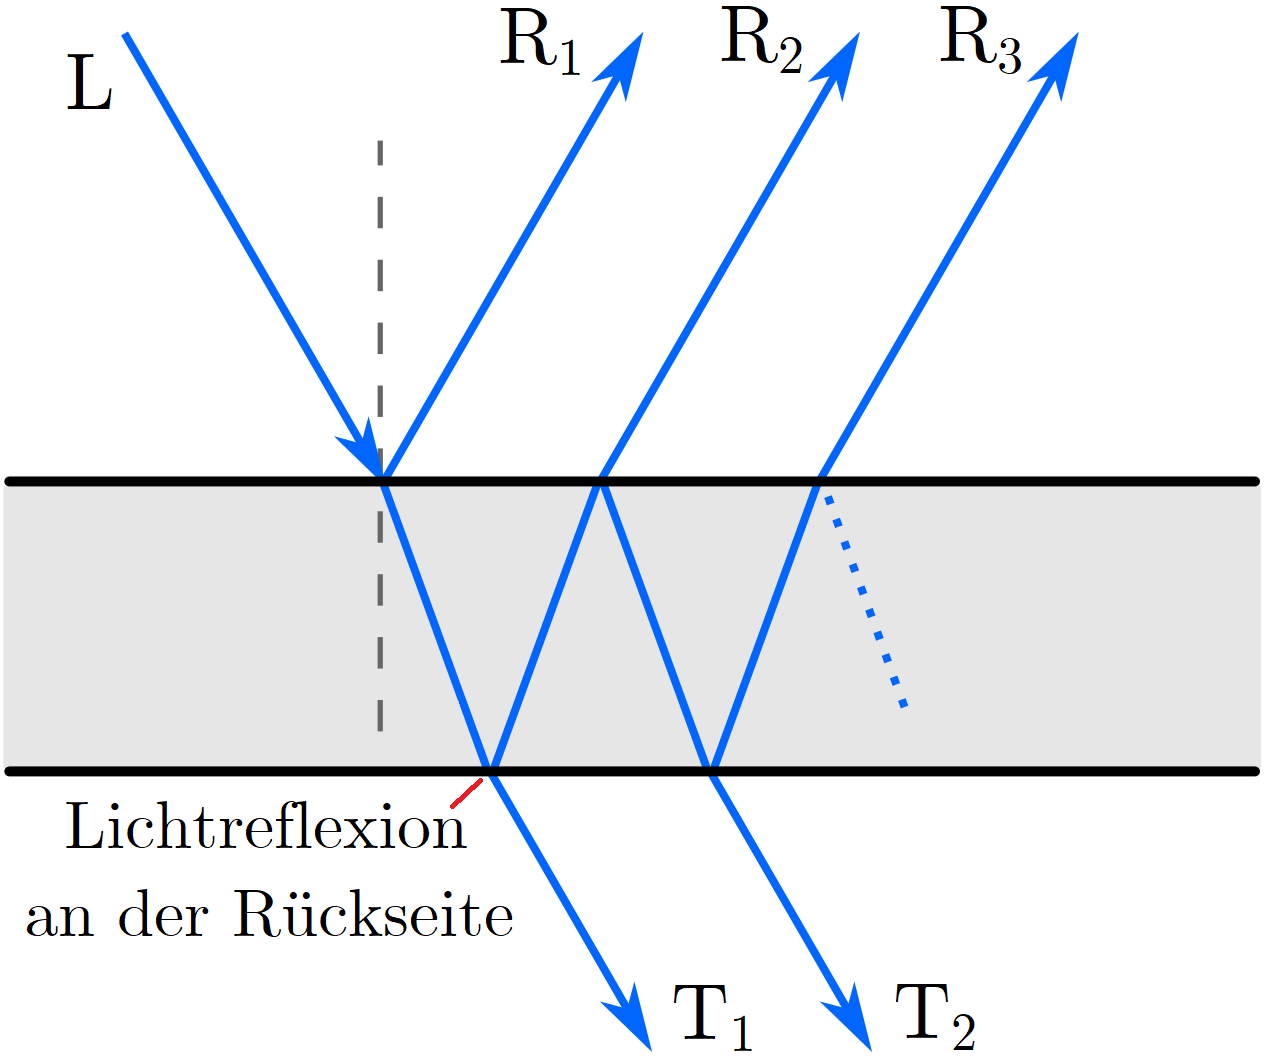
\includegraphics[width=0.75\columnwidth]{rueckseitenreflex}
		\caption{Rückseitenreflex \cite{deflektometrieScheiben}}
		\label{img:rueckseitenreflex}
	\end{figure}
	
	Die Szenen sind entscheidend zur Auswertung, da diese über die Aufnahme in den Bildkanal übertragen werden.
	Über die Szene lassen sich Punkte aus dem Kamerabild und der Szene zuordnen.
	Man erhält durch geeignete Auswertungen eine Zuordnungsfunktion, die beschreibt welcher Kamerapunkt welchen Punkt aus der Szene aufnimmt.
	Die Szene besteht dabei in der Regel aus einem oder mehreren Mustern, die auf einem Bildschirm angezeigt werden (siehe Abb. \ref{img:pruefstation}).
	%
	%img:pruefstation
	\begin{figure}[H]
		\centering
		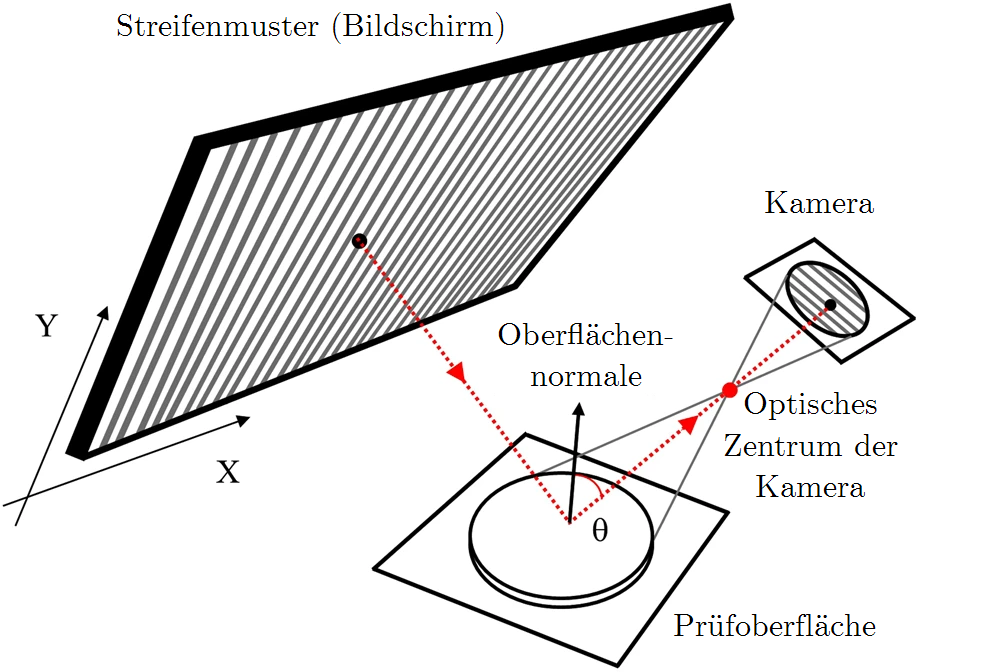
\includegraphics[width=\columnwidth]{nature-articel-nr1}
		\caption{Deflektometrische Prüfstation \cite{aufbau}}
		\label{img:pruefstation}
	\end{figure}
	
	Durch spezielle Lösungen wird es durch die Zuordnungsfunktion ermöglicht, die spiegelnde vollständig Oberfläche zu rekonstruieren.
	Allerdings ist dies eine schwierige mathematische Aufgabe, die viele Parameter und Lösungen für Differentialgleichungen erfordert.
	
	\section{Sichtprüfung durch Lichtstreuung} \label{sec:sichtpruefungDurchLichtstreuung}
	Das erste Verfahren soll es insbesondere für transparente Prüfobjekte ermöglichen, Kratzer und ähnlich Defekte hervorzuheben.
	Dabei wird folgender Aufbau verwendet, um den Rückseitenreflex zu vermeiden:
	%
	%img:durchlichtaufbau
	\begin{figure}[H]
		\centering
		
\includegraphics[width=0.7\columnwidth]{aufbau}
		\caption{Prüfaufbau für transparente Objekte.}
		\label{img:aufbau}
	\end{figure}
	
	Die Idee des Verfahrens ist es, die abweichende Lichtstreuung an Kratzern und ähnlichen Defekten der Oberflächen zu nutzen und durch geeignete Bildverknüpfungen ein Gesamtbild zu erzeugen, dass zur Detektion dieser Defekte dienen kann.
	
	%
	%img:imageTree
	\begin{figure}[H]
		\centering
		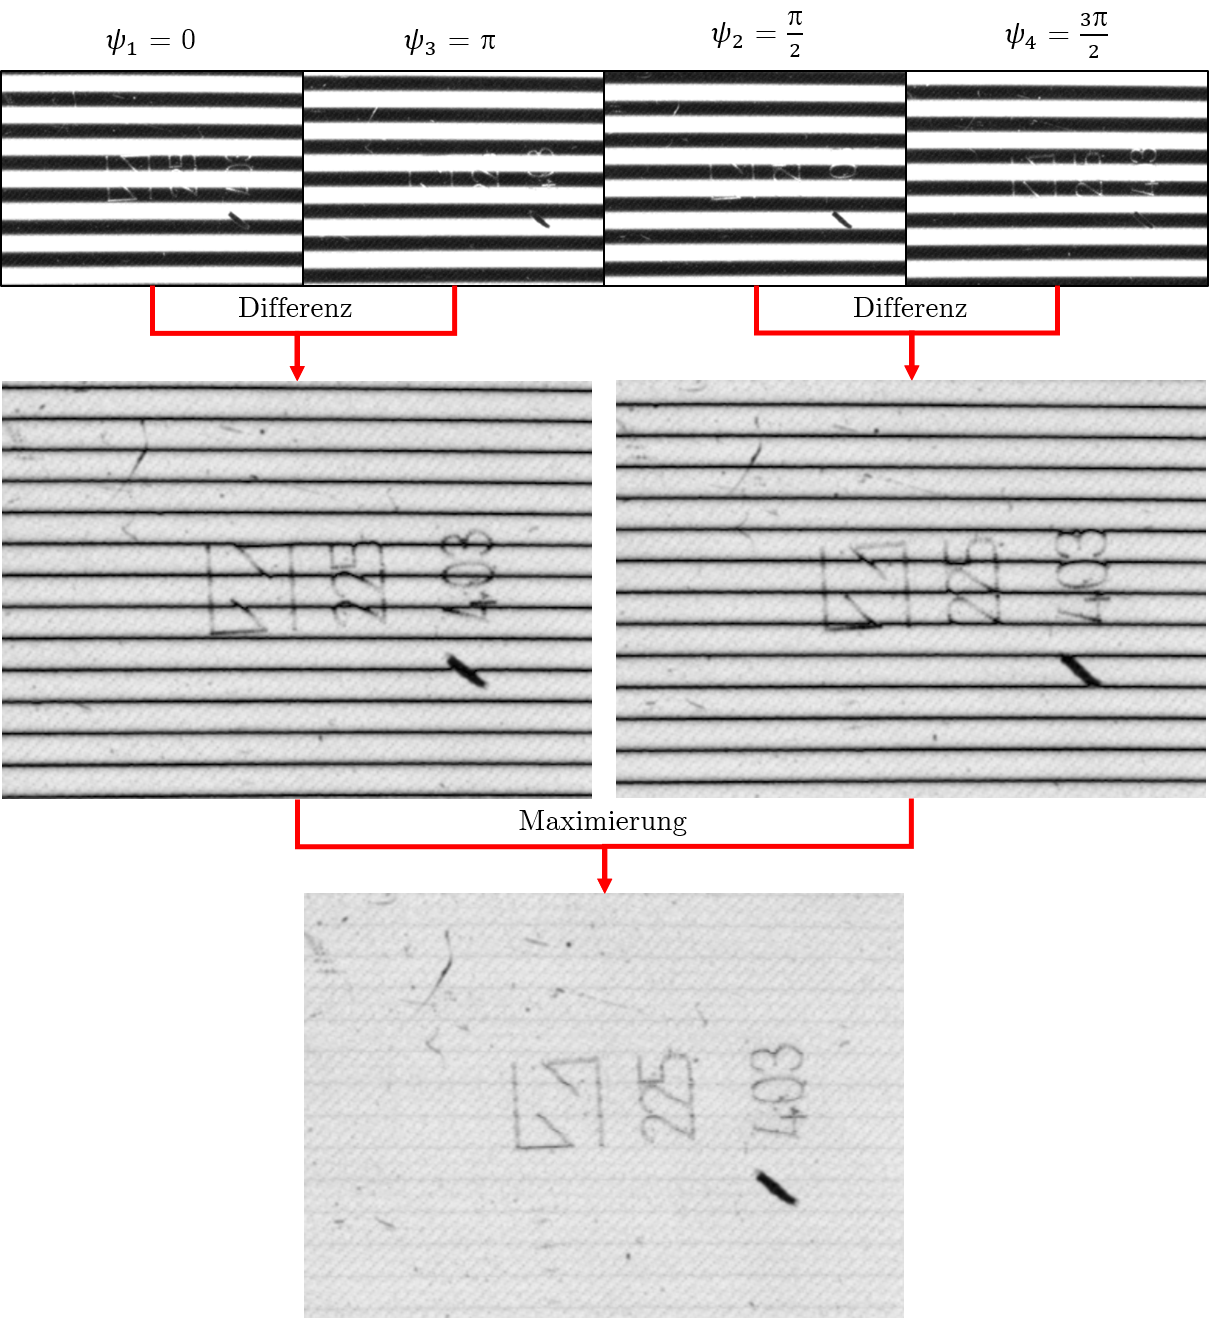
\includegraphics[width=\columnwidth]{imageTree}
		\caption{Vorgehensweise des Verfahrens}
		\label{img:imageTree}
	\end{figure}
	
	In Abb. \ref{img:imageTree} wird die Vorgehensweise des Verfahrens dargestellt.
	Man nimmt Streifenmuster bei der Durchlichtprojektion auf und verknüpft die jeweils um eine Streifenbreite versetzten Muster über die betragsmäßige Differenz.
	Schlussendlich bildet man das Maximumsbild aus allen Bildern.
	
	\par
	Dabei werden Kratzer und stärkere Krümmungen sichtbar.
	Durch geeignete Anpassung des Aufbaus ist dieses Verfahren auch anwendbar für spiegelnde Prüfobjekte.
	
	\section{Deflektometrische Registrierung} \label{sec:deflektometrischeRegistrierung}
	Die deflektometrische Registrierung $l_r$ bezeichnet die in Abschnitt \ref{sec:grundlagenDerDeflektometrie} erwähnte Zuordnungsfunktion von Punkten der Szene und Punkten des Kamerabilds (siehe Abb. \ref{tikz:abbildungssystem}).
	Anhand der deflektometrischen Registrierung soll ein zweites Verfahren zur Auswertung von spiegelnden Oberflächen vorgestellt werden.	
	%
	% tikz:abbildungssystem
	\begin{figure}[H]
		\centering
		\vspace*{-0.5cm} %Positionierung dieses Tikz-Pictures anpassen, da die Stützpunkte des geekrümmten Pfeils außerhalb der tatsächlichen Boundingbox liegen und diese mitzählen.
		\begin{adjustbox}{width=\columnwidth}
		\begin{tikzpicture}[every node/.style={inner sep=0,outer sep=0}]
		
			%Bild der Oberfläche laden
			\node [anchor=north] (imgOberflaeche) at (0,0) {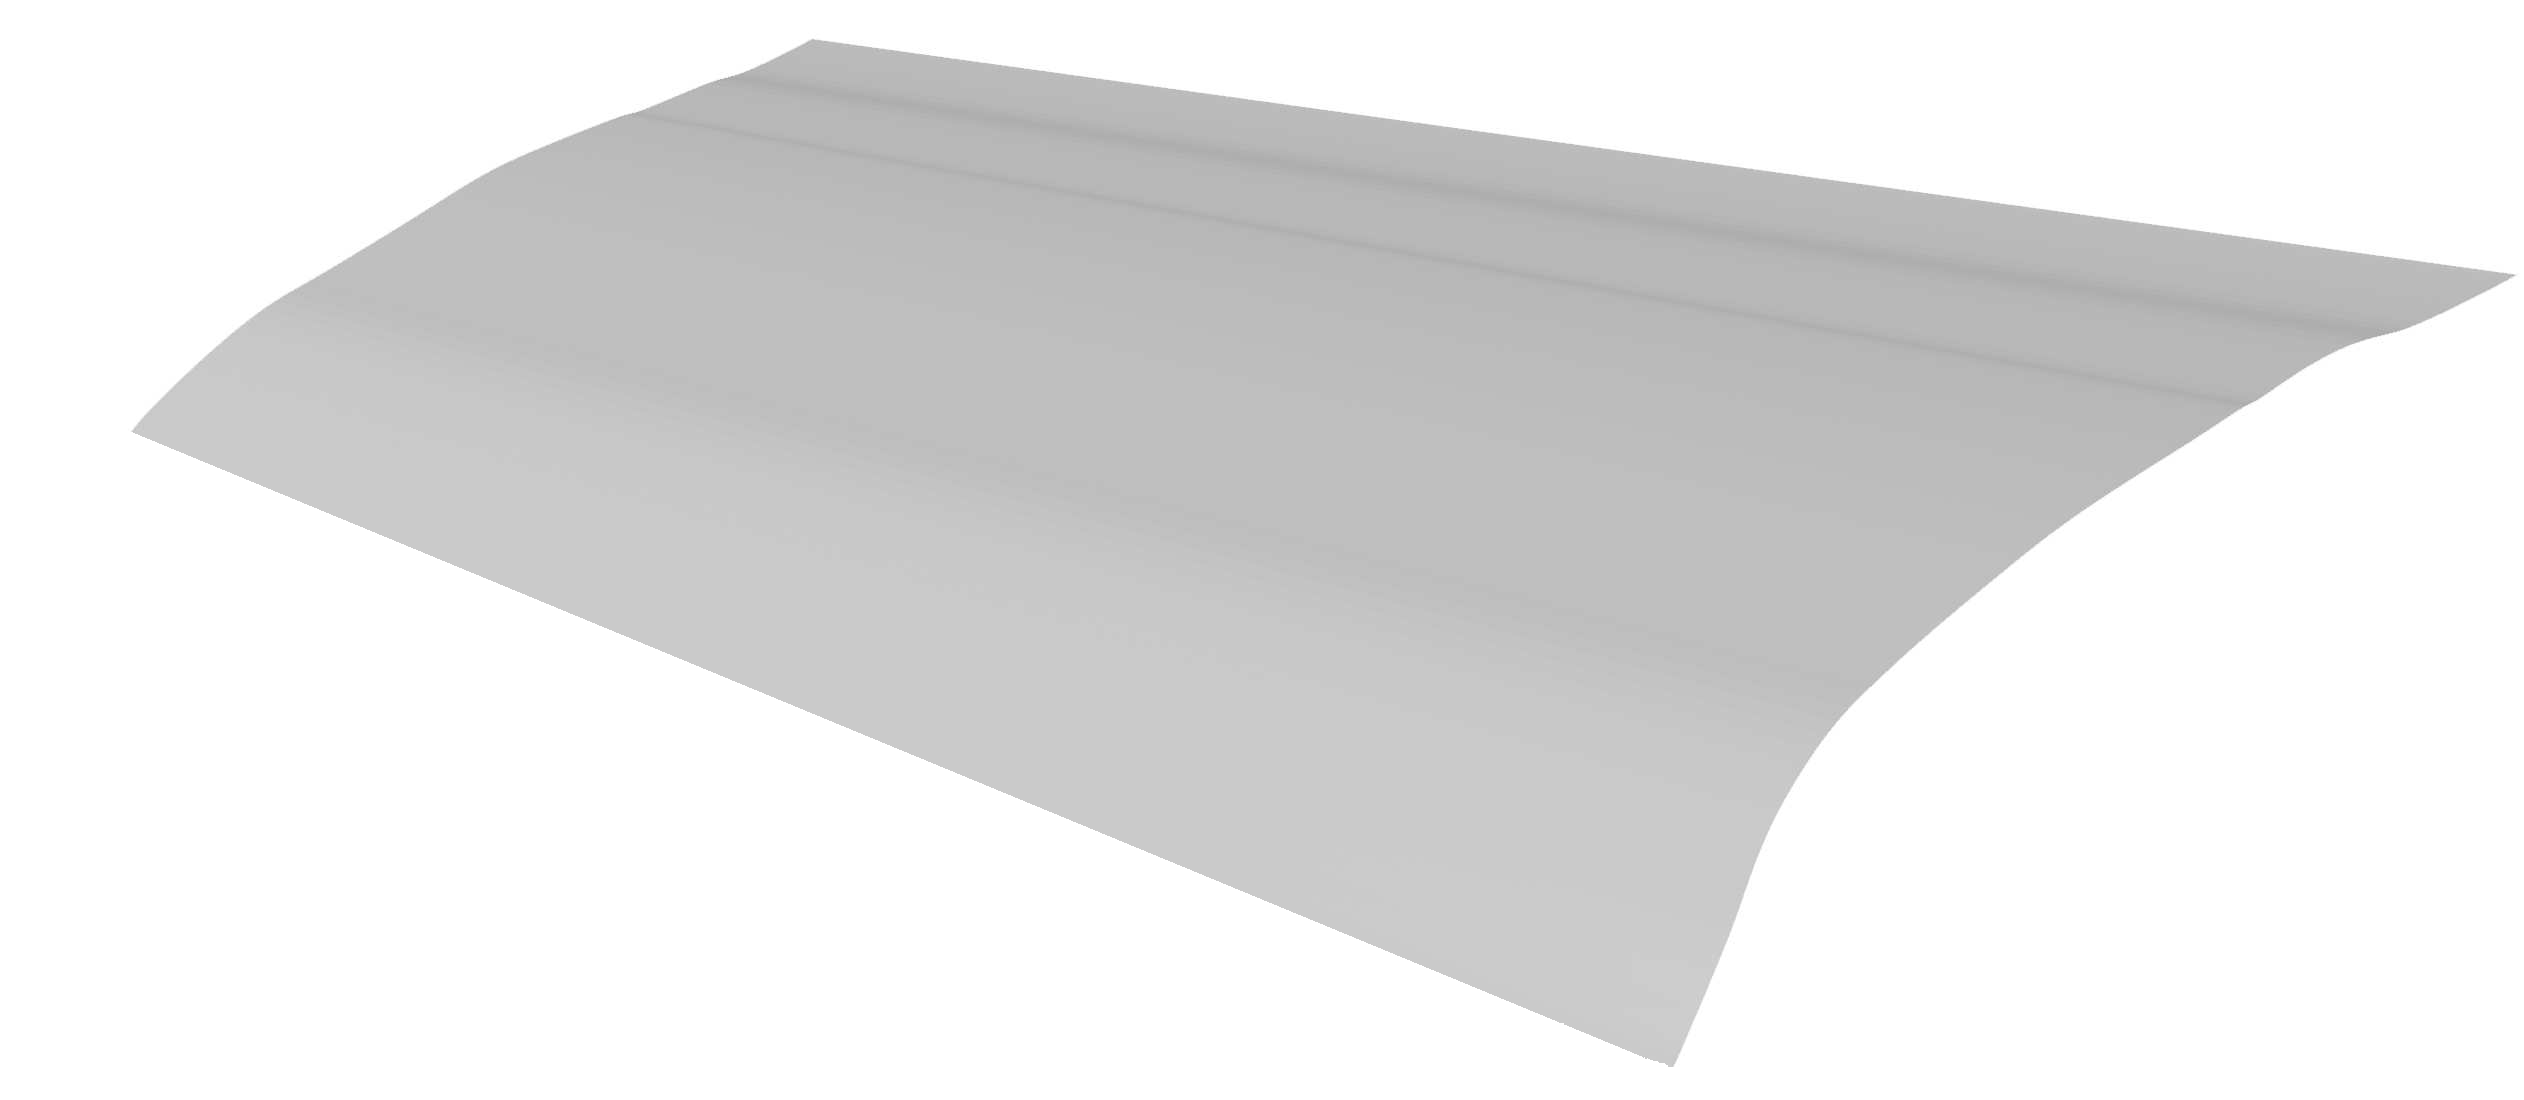
\includegraphics[width=360pt]{oberflaeche}};
			
			%Punkte setzen
			\node (monitorpunkt) at (-6,0) {};
			\node (objektpunkt) at (0,-3) {};
			\node (kamerapunkt) at (4,1.5) {};
			
			%Kamera und Monitor zeichnen
			\node [trapezium, draw, minimum width=1.5cm, minimum height=1cm, trapezium left angle=120, trapezium right angle=60, trapezium stretches=false, inner sep=2] (kamera) at (kamerapunkt) {};
			\node [trapezium, draw, rotate=35, minimum width=1cm, minimum height=1.5cm, trapezium left angle=40, trapezium right angle=140, trapezium stretches=false, inner sep=2, fill=black!5] (monitor) at (monitorpunkt) {};		
			
			%Punkte beschriften
			\node [circle,fill=black,minimum size=5pt] at (monitorpunkt) {};
			\node [circle,fill=black,minimum size=5pt] at (objektpunkt) {};
			\node [circle,fill=black,minimum size=5pt] at (kamerapunkt) {};
			\node [below left=4pt and 2pt of monitorpunkt] {\Large M};
			\node [below=6pt of objektpunkt] {\Large P};
			\node [below right=1pt and 5pt of kamerapunkt] {\Large K};
			
			%Lichtstrahl zeichnen
			\draw[red,very thick,midarrow] (monitorpunkt) -> (objektpunkt);
			\draw[red,very thick,midarrow] (objektpunkt) -> (kamerapunkt);
			
			%Abbildung zeichnen
			\draw[Green,very thick,-{Latex[width=3mm]}] (kamerapunkt) to [out=120, in=60] node[midway,outer sep=4pt,above] {\Large $l_r$} (monitorpunkt);
		
				%Oberflächennormale zeichnen
			\draw[very thick,-{Latex[width=3mm]}] (objektpunkt) --++ (100.5:1.5cm) node[right=5pt] {\Large $n$};
			%Monitor, Oberfläche und Kamera beschriften
			\node[anchor=east] at (-5.5,1.7) {\Large Bildschirm};
			\node[anchor=west] at (3.9,0.6) {\Large Kamerasensor};
			\node[anchor=west] at (3.2,-4.1) {\Large Oberfläche};
			
			\end{tikzpicture}
		\end{adjustbox}
		\caption{Abbildungssystem einer spiegelnden Oberfläche}
		\label{tikz:abbildungssystem}
	\end{figure}
	
	In dieser Arbeit wird die Bestimmung der deflektometrischen Registrierung über die Phasenkodierung durchgeführt.
	Dabei werden die Punkte des Monitors, über die Phase von Sinus-Funktionen kodiert, in den Bildkanal der Kamera übertragen.
	Die verwendeten Muster werden als sinusoidale Streifenmuster bezeichnet (siehe Abb. \ref{img:sinusoidalesMuster}).
	%
	% img:sinusoidalesMuster
	\begin{figure}[H]
		 \centering
		 
\includegraphics[frame,width=0.4\columnwidth]{m_1_3}
		 \caption{Sinusoidales Streifenmuster}
		 \label{img:sinusoidalesMuster}
	\end{figure}
	
	Durch bestimmte Methoden lassen sich die Phasen des gespiegelten Streifenmusters bestimmen, wodurch man die Zuordnung erhält.
	
	\par
	Es ist möglich durch Separierung der Zuordnung in eine Zeilen- und eine Spaltenzuordnung, diese als Bilder darzustellen.
	Dadurch kann man herkömmliche Bildverarbeitung anwenden um Fehlstellen zu detektieren (siehe Abb. \ref{tikz:gradientenAuswertung}).
	
	\begin{figure}[H]
		\centering
		\begin{adjustbox}{width=\columnwidth}
			\begin{tikzpicture}[every node/.style={inner sep=0,outer sep=0}]
			
				\node [anchor=north east] (imgSpalten) at (-0.03\columnwidth,0) {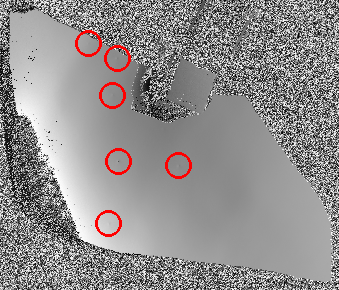
\includegraphics[width=.47\columnwidth]{pickelDeflektometrischeRegistrierung}};
				\node [below=0.2cm of imgSpalten, align=center] {\footnotesize Graubild der \\ \footnotesize Spaltenzuordnung};
				\node [anchor=north west] (imgGradienten) at (0.03\columnwidth,0) {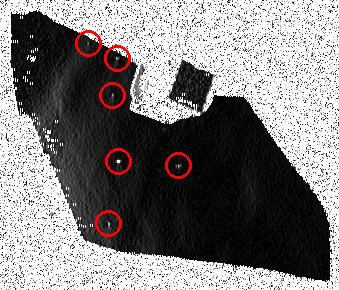
\includegraphics[width=.47\columnwidth]{pickelGradientenbild}};
				\node [below=0.2cm of imgGradienten, align = center] {\footnotesize Bild der Ableitung \\ \footnotesize des linken Graubilds};
				
			\end{tikzpicture}
		\end{adjustbox}
		\caption{Spaltenzuordnung eines spiegelnden Objekts als Bild und dessen Ableitung in $x$-Richtung. In Rot: Pickel als Fehlstellen auf der Oberfläche}
		\label{tikz:gradientenAuswertung}
	\end{figure}

	Im Vergleich zur vollständigen Rekonstruktion der Oberfläche, ist es durch die deflektometrische Registrierung möglich, die Krümmung der Oberfläche ohne eine Systemkalibrierung auszuwerten.
	
	\section{Ergebnisse} \label{sec:ergebnisse}
	
	
	\section{Abschlussbemerkungen} \label{sec:abschlussbemerkungen}
	
	% Quellenverweise
	\printbibliography[title = Quellenverzeichnis]
\end{document}
%-DOKUMENT-Ende-----------------------------------------------------------
